\documentclass[12pt]{standalone}

\usepackage{tikz}

\tikzset{real edge/.style={solid,very thick}}
\tikzset{virtual edge/.style={dashed,thin}}

\begin{document}
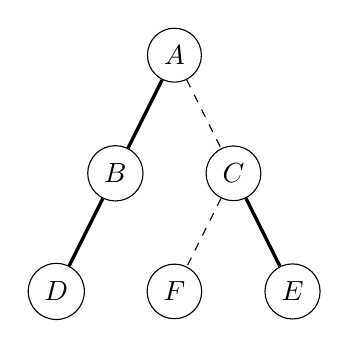
\begin{tikzpicture}

\scoped[every node/.style={solid,thin,circle,draw}]
\node (A) {$A$}
    child[real edge] {node (B) {$B$}
        child[real edge] {node (D) {$D$}}
        child[missing]}
    child[virtual edge] {node (C) {$C$}
        child[virtual edge] {node (F) {$F$}}
        child[real edge] {node (E) {$E$}}};

\end{tikzpicture}
\end{document}
